% Chapter 7

\chapter{Design Decisions \& Implementation Details}

\label{ch:design}

%----------------------------------------------------------------------------------------

\section{Pairwise Iterator} \label{sec:design:pairwise}

The pairwise iterator (in \texttt{tangible/utils.py}, see section
\ref{subsec:architecture:pairwise}) has an interesting implementation that might
not be immediately obvious to someone new to Python and its standard library:

\vspace{.5\baselineskip}
\begin{pythoncode}
from itertools import tee, izip

def pairwise(iterable):
    a, b = tee(iterable)
    next(b, None)
    return izip(a, b)
\end{pythoncode}

\noindent The \texttt{tee(iterable, n)} function returns \texttt{n} independent
iterators from a single iterable. The default value for \texttt{n} is
\texttt{2}, so in the example above two iterators called \texttt{a} and
\texttt{b} are created from the original iterable.

The second iterator is then advanced once by applying the \texttt{next()}
function to it. The return value is discarded. This results in two iterators,
one of them with an offset of 1.

As a last step, the two iterators are zipped together. By using the
\texttt{izip()} function instead of the regular \texttt{zip()}, a lazy generator
is returned instead of a list. This decreases memory consumption, especially
when handling large lists.

Now each time the returned generator is advanced one step, the sliding window is
shifted by 1 position and the resulting tuple is returned, until the end of the
iterator is reached.

\vspace{.5\baselineskip}
\begin{pythoncode}
>>> data = [1, 2, 3, 'a']
>>> pairs = pairwise(data)
>>> pairs
<itertools.izip object at 0x151def0>
>>> next(pairs)
(1, 2)
>>> next(pairs)
(2, 3)
>>> next(pairs)
(3, 'a')
>>> next(pairs)
Traceback (most recent call last):
  File "<stdin>", line 1, in <module>
	StopIteration
\end{pythoncode}

%----------------------------------------------------------------------------------------

\section{Code Generation} \label{sec:design:codegen}

Code generating code is often something quite messy, with many conditionals and
a lot of \texttt{print} statements and string formatting. Such an approach is
both hard to read and hard to maintain. Additionally, it does not reflect the
structure of the generated code.

In the OpenSCAD backend implementation, \tangible{} uses an approach proposed by
Tomer Filiba \cite{filiba:2012}, which builds upon Python's context managers to
generate nested blocks of code.

\marginpar{Context Managers are Python constructs that create a runtime context
for a piece of code when used in combination with the \texttt{with} statement.
They provide enter- and exit-hooks that are invoked before and after executing
that code.}

There is a top level class called \texttt{Program} which exposes a
\texttt{statement} method and a \texttt{block} context manager. The class holds
a stack of blocks and a list of child blocks and statements. Each time a block
is entered (by using a \texttt{with}-statement), it is pushed to the stack and
appended to the list of children. When leaving the context manager, the block is
removed again from the stack.

The final code is generated by walking the list of children in the
\texttt{Program} instance recursively. This is also the point where
language-specific features can be implemented, for example indentation of a
block in Python or inserting curly braces in Java or C.

A special feature that was implemented in the code generation is the support for
predefined code snippets to be included in the generated output. This part of
the code is called the ``preamble''. Snippets can be inserted into the preamble
multiple times, but they're rendered only once. This has proven to be very
useful while implementing code generation for circle sectors (see section
\ref{sec:design:circlesectors}).

Right now all the described classes are contained in the OpenSCAD backend. By
generalizing the code, it would be possible to create a base class for all code
generation backends, with the possibility to configure the language-specific
details in a single subclass. This might be a good idea for a future version of
\tangible{}.

An extract from the actual code which decides how the AST is mapped to the
backend syntax is shown on the next page.

\vspace{.5\baselineskip}
\begin{pythoncode}
class OpenScadBackend(object):
    """Render AST to OpenSCAD source code."""

    def __init__(self, ast):
        self.ast = ast

    def generate(self):
        prgm = Program()
        BLOCK = prgm.block
        STMT = prgm.statement
        PRE = prgm.preamble
        SEP = prgm.emptyline

        def _generate(node):
            """Recursive code generating function."""

            istype = lambda t: node.__class__ is t

            # Handle lists
            if istype(list):
                for item in node:
                    _generate(item)

            # Simple statements
            elif istype(ast.Circle):
                STMT('circle({0})', node.radius)
            elif istype(ast.Rectangle):
                STMT('square([{0}, {1}])', node.width, node.height)

            # Blocks
            elif istype(ast.Union):
                with BLOCK('union()'):
                    _generate(node.items)

            # (...)

        _generate(self.ast)

        return prgm.render()
\end{pythoncode}

%----------------------------------------------------------------------------------------

\newpage
\section{Circle Sectors in OpenSCAD}\label{sec:design:circlesectors}

By default, OpenSCAD does not support circle sectors. Therefore the shape had to
be developed manually as a module.

\vspace{.5\baselineskip}
\begin{minted}[frame=lines,framesep=2mm,samepage=true,fontsize=\footnotesize]{javascript}
module circle_sector(r, a) {
    a1 = a % 360; a2 = 360 - (a % 360);
    if (a1 <= 180) {
        intersection() {
            circle(r);
            polygon([
                [0,0],
                [0,r],
                [sin(a1/2)*r, r + cos(a1/2)*r],
                [sin(a1)*r + sin(a1/2)*r, cos(a1)*r + cos(a1/2)*r],
                [sin(a1)*r, cos(a1)*r],
            ]);
        }
    } else {
        difference() {
            circle(r);
            mirror([1,0]) {
                polygon([
                    [0,0],
                    [0,r],
                    [sin(a2/2)*r, r + cos(a2/2)*r],
                    [sin(a2)*r + sin(a2/2)*r, cos(a2)*r + cos(a2/2)*r],
                    [sin(a2)*r, cos(a2)*r],
                ]);
            };
        }
    }
};
\end{minted}

\noindent The base concept is a boolean combination of a circle and a polygon,
depending on the angle. If the angle is less than or equal to 180\si{\degree},
the resulting shape is the intersection of the circle and the polygon. If it's
larger than 180\si{\degree}, the difference between the two shapes is returned.

The polygon always consists of five points, which are calculated as shown in the
following table for angles less or equal to 180\si{\degree}. For angles between
180\si{\degree} and 360\si{\degree}, the polygon is simply mirrored along the y
axis.

\begin{table}[H]
	\centering
	\begin{tabularx}{\textwidth}{XX} \toprule
		\tableheadline{x} & \tableheadline{y} \\
		\midrule
		$0$ & $0$ \\
		$0$ & $r$ \\
		$\sin(\alpha / 2) \cdot r$ & $r + \cos(\alpha / 2) \cdot r$ \\
		$\sin(\alpha) \cdot r + \sin(\alpha / 2) \cdot r$ & $\cos(\alpha) \cdot r + \cos(\alpha / 2) \cdot r$ \\
		$\sin(\alpha) \cdot r$ & $\cos(\alpha) \cdot r$ \\
		\bottomrule
	\end{tabularx}
\end{table}

\noindent The following six images show the circle and polygon combinations for
45, 90, 180, 225, 270 and 315 degrees.

\begin{figure}[H]
	\centering
	\subfloat[]{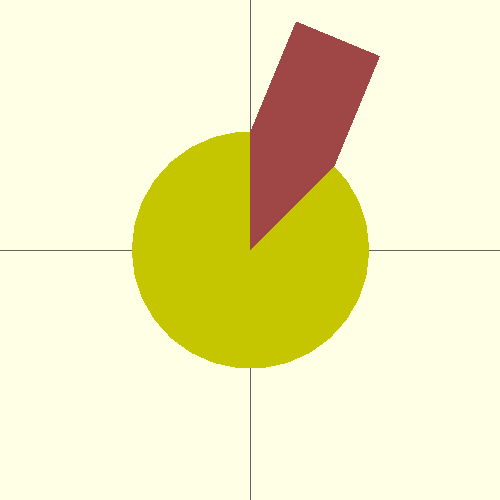
\includegraphics[width=.30\textwidth]{images/cs_45}}
	\quad
	\subfloat[]{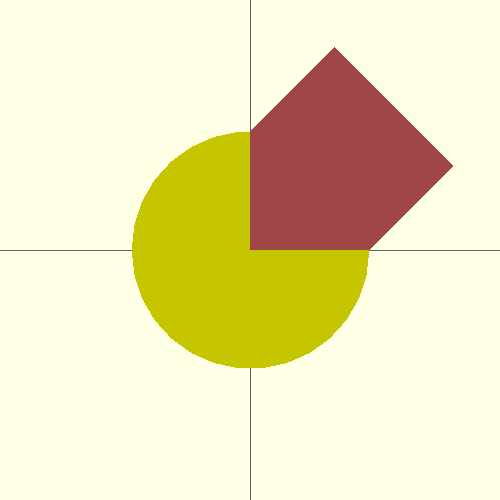
\includegraphics[width=.30\textwidth]{images/cs_90}}
	\quad
	\subfloat[]{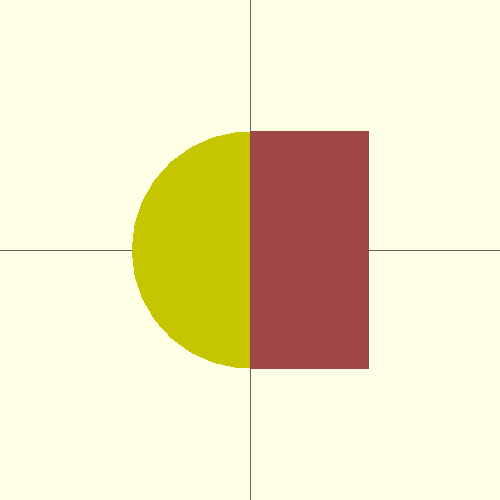
\includegraphics[width=.30\textwidth]{images/cs_180}}
	\\
	\subfloat[]{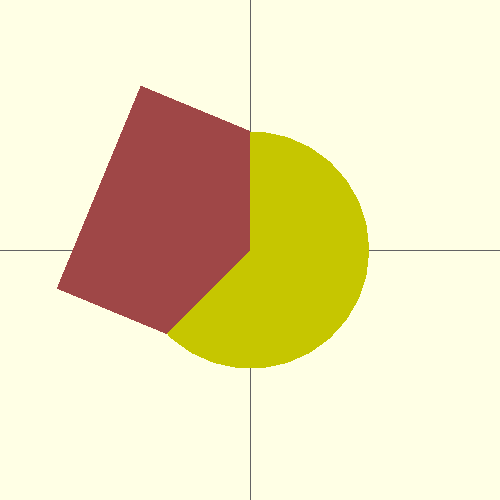
\includegraphics[width=.30\textwidth]{images/cs_225}}
	\quad
	\subfloat[]{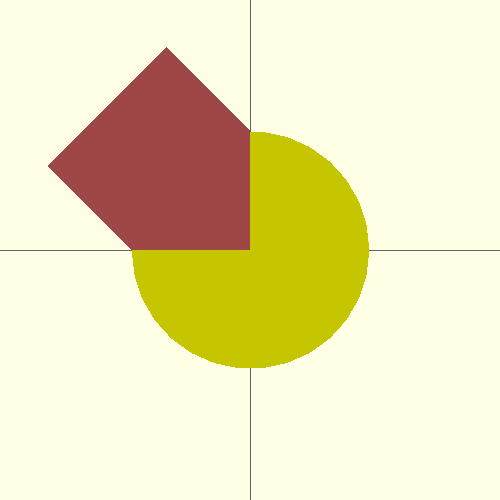
\includegraphics[width=.30\textwidth]{images/cs_270}}
	\quad
	\subfloat[]{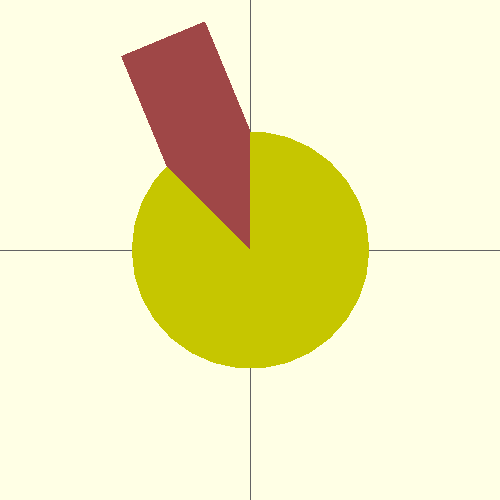
\includegraphics[width=.30\textwidth]{images/cs_315}}

	\caption{Circle and polygon combinations at different angles}
	\label{img:circle_shape_angles}
\end{figure}

\noindent By combining the two shapes in such a way, any circle sector can be
created. Example for \texttt{circle\_sector(10, 225)}:

\begin{figure}[H]
	\centering
	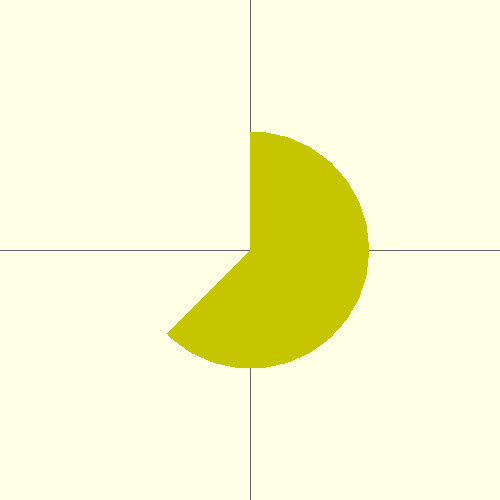
\includegraphics[width=.70\textwidth]{images/cs_225_result}
	\caption{The resulting circle sector for an angle of 225\si{\degree}}
	\label{img:circle_shape_result}
\end{figure}

\noindent The module source code is used in the OpenSCAD backend implementation
as a preamble snippet.
